\documentclass[a4paper, 12pt]{article}
\def\xcolorversion{2.00}
\def\xkeyvalversion{1.8}

%\usepackage[utf8]{inputenc} 
\usepackage[frenchb]{babel}
\usepackage{fullpage}
\usepackage[T1]{fontenc} 
\usepackage{graphicx}  
\usepackage[final]{pdfpages}
\usepackage{amsmath, amssymb,amsthm}
\usepackage{algorithm,algorithmic}
\usepackage{listingsutf8}
\usepackage{lmodern}
\usepackage[tikz]{bclogo}
\usetikzlibrary{arrows,shapes,snakes,automata,backgrounds,petri}
%\usepackage[version=0.96]{pgf}
\usepackage{pgfplots}
\usepackage{fancybox}
\usepackage{makecell}
\usepackage{array, multirow, tabularx}
\usepackage{xcolor}
\usepackage{framed, color}
\setlength{\parskip}{\bigskipamount}


\newtheorem{mydef}{Définition}
\newtheorem{thm}{Théorème}
\newtheorem{lem}{Lemme}
\newtheorem{cor}{Corollaire}
\newtheorem{prop}{Propriété}
\newtheorem{conj}{Conjecture}

\title{TP M2: Réseaux de Pétri} \author{William Dyce, Amal Mejdoub, Sabrina Ouazzani-Chahdi} 

\date{Décembre/Janvier 2012/2013}

\begin{document}

\newcommand\bcdef{
\includegraphics[width=0.6cm]{def.png}}

\maketitle

\begin{bclogo}[couleur=blue!15, arrondi=0.1, logo= \bcdef,
    ombre=true, epOmbre=0.25, couleurOmbre=black!30, epBarre=1,
    barre=zigzag]{Résumé} Le présent rapport est le compte-rendu du
  projet TP d'Ingénierie des protocoles du M2 Informatique de
  l'Université Montpellier II.
\end{bclogo}

\section{Exercice 1 : L'utilisation des réseaux de Pétri pour le
  contrôle commande}
\subsection{Question 1}
\textit{Cf.} figure $3$ de l'énoncé.
\subsection{Question 2}
Notons $A_d$ et $R_d$ respectivement avancer et reculer le pochoir de
droite.  Notons $A_g$ et $R_g$ respectivement avancer et reculer le
pochoir de gauche.  Quand un pochoir avance, il ne recule pas.  On
commence donc pas le faire avancer ($p_3$ et $p_2$) puis reculer
($p_4$ et $p_5$) On distingue un bloc de parallélisme dans la figure 3
qui signifie que les pochoirs droite et gauche sont actionnés en
parallèle.

Au début d'un tour, en $p_1$, le pochoir ne reçoit aucun signal.  

Puis, en $t_1$, l'opération commence car on a les signaux $p$ et $q$ à
vrai. On rentre ensuite dans le bloc de parallélisme précédemment
décrit, jusqu'à $t_6$ où, après immobilisation à droite et à gauche
des pochoirs (places $p_6$ et $p_7$), un nouveau tour peut commencer
(retour en place $p_1$).
\subsection{Question 3}
Le réseau de la figure $3$ est cohérent. En effet, de $p_1$ à $t_1$ un
seul jeton est en circulation. De $t_1$ à $t_6$ deux jetons sont en
circuation, mais dans une structure de type parallélisme (un jeton par
branche). En $t_6$, pour le retour à $p_1$, un seul jeton est à
nouveau en circulation. Chaque place ne reçoit donc qu'une seule
marque tout au long des évolutions du réseau.
\subsection{Question 4}
Les combinaisons booléennes des signaux de sorties incompatibles sont
situées de manière séquentielle (et non parallèle). De plus, le réseau
est cohérent. Cela nous garantit ainsi l'exclusion mutuelle pour tous
les couples de places associés à ces étiquettes.
\subsection{Question 5}
Le graphe des marquages accessibles associé au réseau de la figure $3$
est le suivant~:
$(p_1, p_2, p_3, p_4, p_5, p_6, p_7)$

**************************************

(sommet $0$) $(1, 0, 0, 0, 0, 0, 0)$

(a pour voisin)

(sommet $1$) $(0, 1, 1, 0, 0, 0, 0)$

(a pour voisin)

(sommet $2$) $(0, 0, 0, 1, 1, 0, 0)$

(a pour voisin)

(sommet $3$) $(0, 0, 0, 0, 0, 1, 1)$

et retour à sommet $0$.

\subsection{Question 6}
Matrice $C$ d'incidence du réseau de pétri de la figure $3$.

 $ \begin{pmatrix}
C&t_1&t_2&t_3&t_4&t_5&t_6 \\
p_1& -1&0&0&0&0&1 \\
p_2&1&-1&0&0&0&0 \\
p_3&1&0&-1&0&0&0 \\
p_4&0&1&0&-1&0&0 \\
p_5&0&0&1&0&-1&0 \\
p_6&0&0&0&0&1&-1 \\
p_7&0&0&0&1&0&-1 
\end{pmatrix}$

\subsection{Question 7}
TODO
\subsection{Question 8}
TODO
\subsection{Question 9}
graphe d'évènements ????
TODO

\pagebreak
\section*{Exercice 2~: Spécification d'un protocole de communication}
\subsection*{Question 1}
\begin{center}
\begin{tikzpicture}[node distance=2cm,>=stealth',bend angle=45,auto]

  \tikzstyle{place}=[circle,thick,draw=blue!75,fill=blue!20,minimum size=6mm]
  \tikzstyle{red place}=[place,draw=red!75,fill=red!20]
  \tikzstyle{transition}=[rectangle,thick,draw=black!75,
  			  fill=black!20,minimum size=4mm]

  \tikzstyle{every label}=[red]

  \begin{scope}
    \node [place, tokens=1] (rac)      [label=above:$u-raccroche$] {};
    \node [place] (dem)      [below of=rac, label=above:$u-demLigne$]{};
    \node [transition] (acc) [below right of=dem,label=right:$acceptation$] {};
    \node [place] (conf)      [above right of=acc, label=above:$c-ConfRac$] {};
    \node [place, tokens=1] (rep)   [above of=conf,label=above:$c-repos$] {};
    \node [place] (com)  [below of=acc, label=right:$enComm$]{};
    \node [transition] (udec) [left of=rac,label=left:$uDecroche$] {};
    \node [transition] (racprem) [left of=dem,label=left:$raccPrem$] {};
    \node [transition] (confrep) [right of=rep,label=right:$confRep$]{};
    \node [transition] (racCom) [left of=com,label=left:$racCom$] {};
    \node [transition] (libe) [below of=com,label=right:$liberation$] {};
    \node [place] (faux)  [below of=libe, label=right:$enFauxAppel$] {};
    \node [transition] (racfaux) [below of=faux,label=below:$racFauxAppel$] {};

    \path[every node/.style={font=\sffamily\small}]
    (acc) 
    edge [pre] (rep)
    edge[pre](dem)
    edge [post] (com)

    (udec)
    edge [pre]                  (rac)
    edge [post]                (dem)

    (confrep)
    edge [pre]                  (conf)
    edge [post]                (rep)

    (racprem) 
    edge [pre]                  (dem)
    edge [post]                (rac)

    (racCom)
    edge [pre]                  (com)
    edge [post,bend right = 20]                (conf)
    edge [post,bend right]                (rac)

    (libe)
    edge [pre]                  (com)
    edge [post]                (faux)

    (racfaux)
    edge [pre]                  (faux)
    edge [post,bend left = 95]                (rac)
    edge [post,bend right = 85]                (conf);

  \end{scope}
  
\end{tikzpicture}
\end{center}

\subsection*{Question 2}

On veut que le réseau soit borné, cohérent et réinitialisable. Nous le
montrons par un Divide Et Impera informel. Commençons par distinguer
trois sous-réseaux~:
\begin{itemize}
\item le réseau utilisateur,
\item le réseau contrôleur,
\item le réseau synchronisé.
\end{itemize}

% insert image schématique du réseau hierarchique

Nous pouvons constater pour commencer que les jetons ne sont pas
dupliqués à l'intérieur de ces réseaux. Remarquons ensuite que le
jeton de chacun des deux réseaux parallèles ne quitte son réseaux
que de manière synchronisée avec l'autre, en passant par la transition
\textsc{acceptation}, et que cette transition produit un unique jeton
dans le réseau synchronisé.
Une fois un jeton dans le réseau synchronisé, il ne peut le quitter
qu'en produisant un jeton dans chacun des réseaux parallèles, par le
bias de \textsc{racrochage-en-communication} ou bien
\textsc{racrochage-en-faux-appel}.
Nous pouvons donc conclure que le réseau et borné et réinitialisable,
et possède soit $1$, soit $2$ jetons, suivant s'il est en mode synchronisé ou en mode parallèle~:
\begin{itemize}
\item $1$ dans chaque réseau parallèle, ou 
\item $1$ dans le réseau synchronisé.
\end{itemize} 
Nous n'avons alors qu'au plus un jeton dans chaque sous-réseau, et de
ce fait le réseau est forcément cohérent.

\subsection*{Question 3}

Matrice $C$ d'incidence du réseau de pétri.

TODO !!!!!!! (just an example below)
 $ \begin{pmatrix}
C&t_1&t_2&t_3&t_4&t_5&t_6 \\
p_1& -1&0&0&0&0&1 \\
p_2&1&-1&0&0&0&0 \\
p_3&1&0&-1&0&0&0 \\
p_4&0&1&0&-1&0&0 \\
p_5&0&0&1&0&-1&0 \\
p_6&0&0&0&0&1&-1 \\
p_7&0&0&0&1&0&-1 
\end{pmatrix}$
\subsection*{Question 4}

TODO

\pagebreak
\section*{Exercice 4~: Spécification d'une construction d'une maison}
\subsection*{Question 1}
\begin{figure}[h!]
\begin{center}
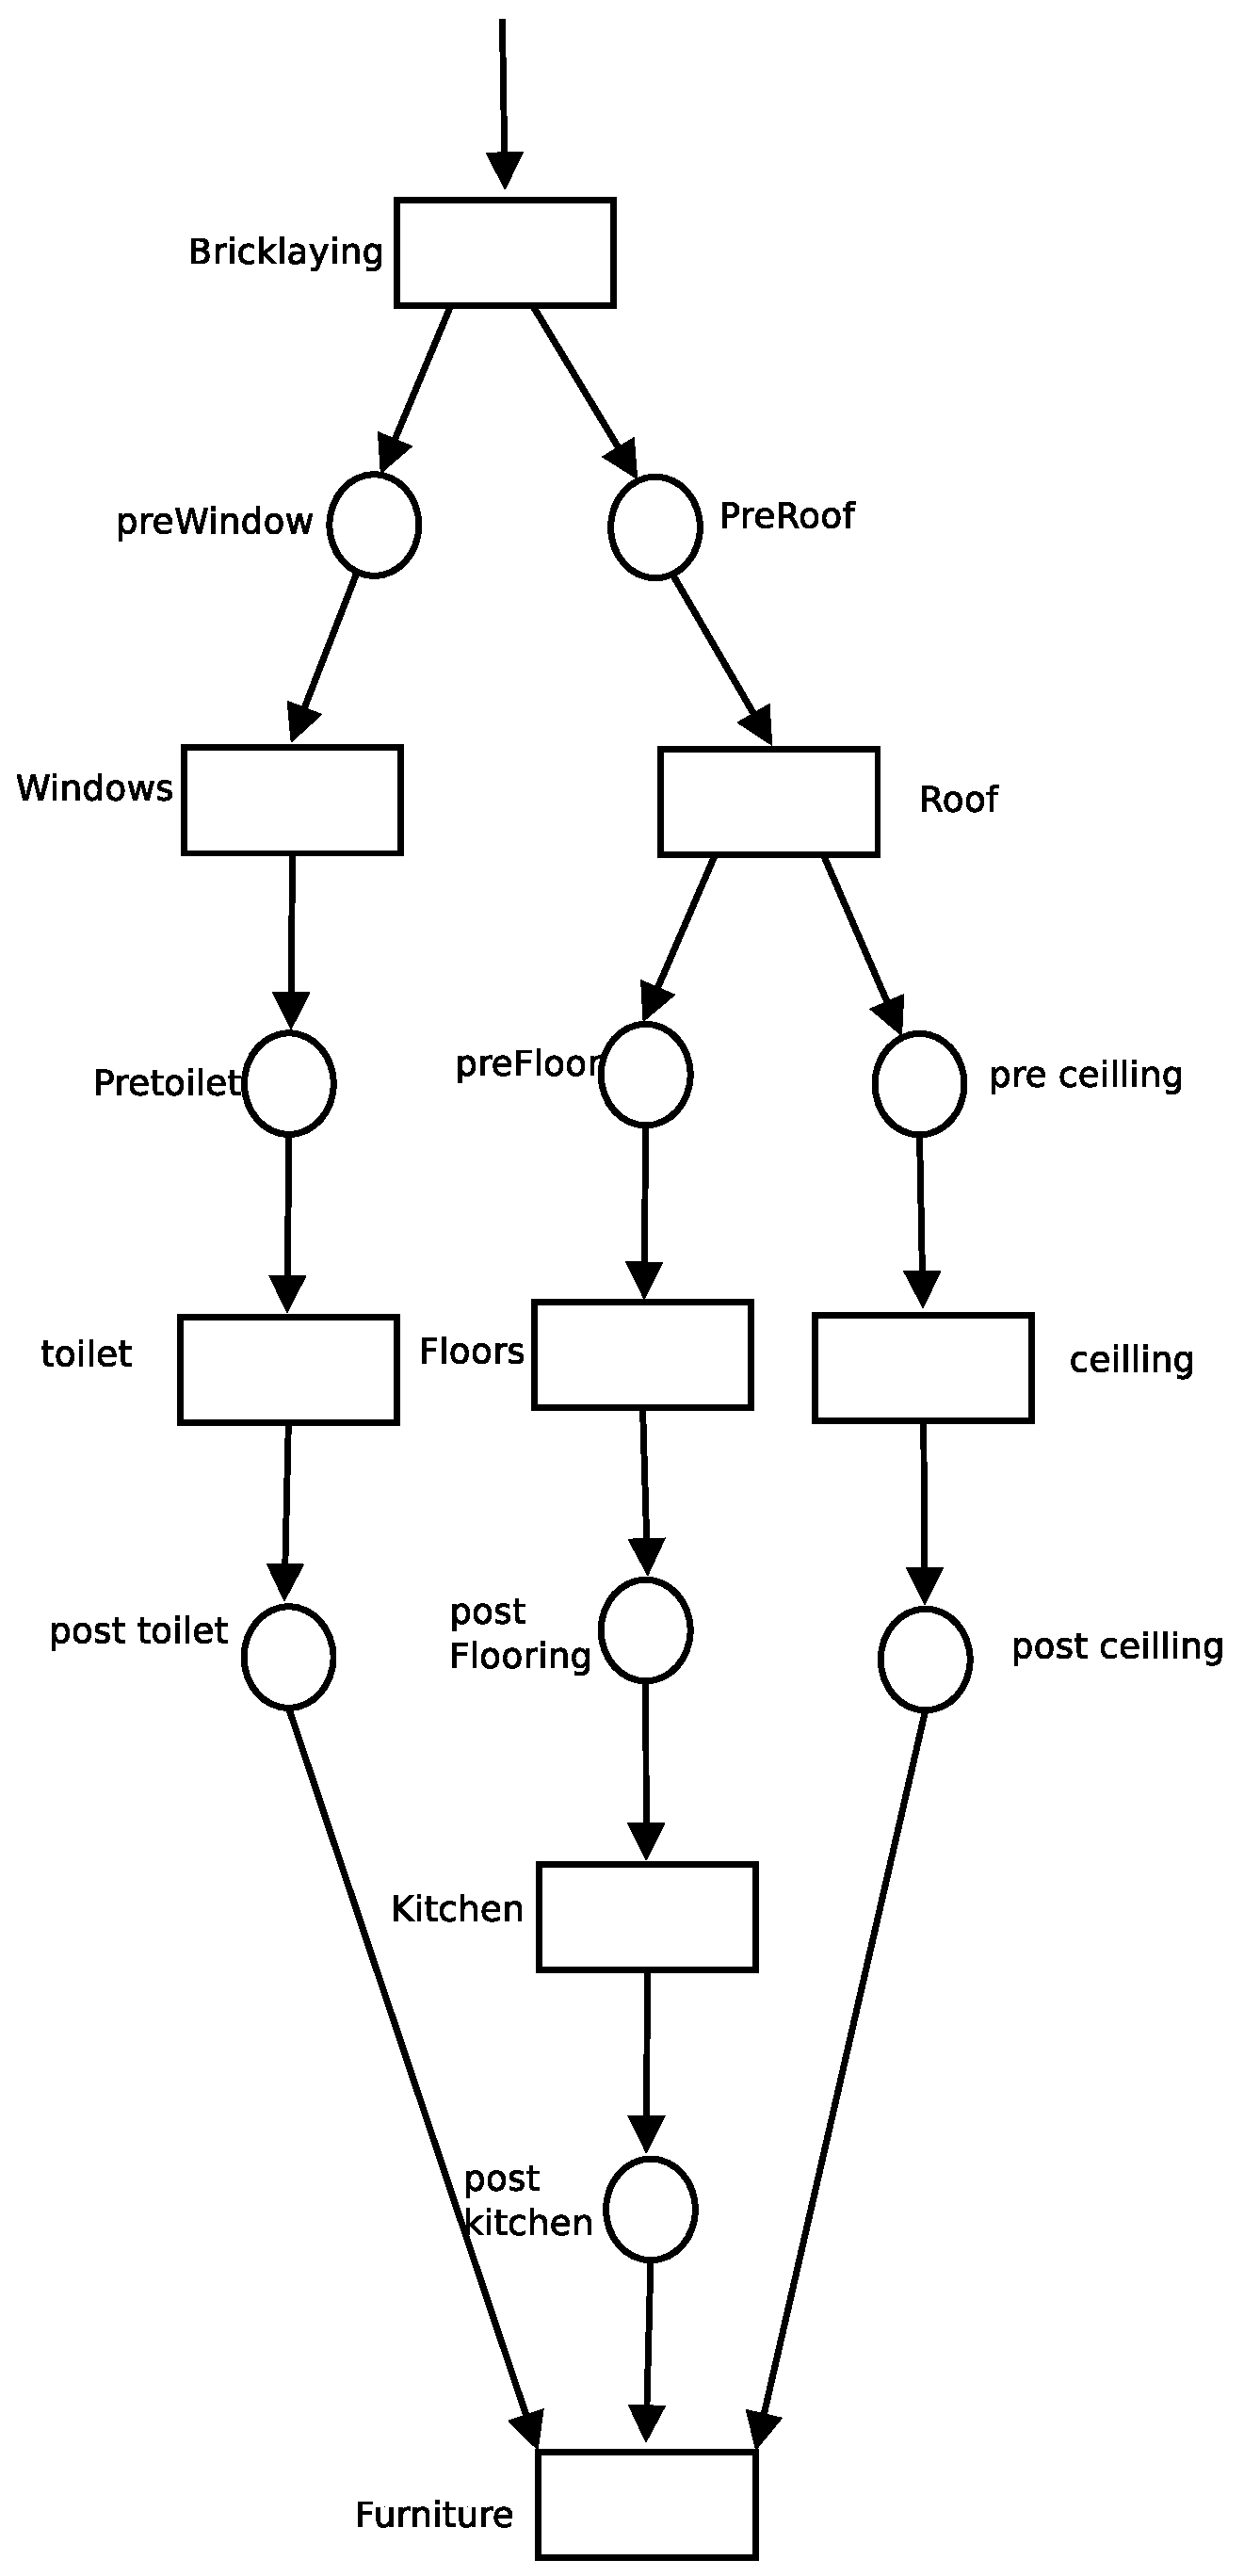
\includegraphics[height = 10cm]{exo41.eps} 
\caption{PT-net where each task is represented by a transition}
\end{center} 
\end{figure} 
\subsection*{Question 2}
\begin{figure}[h!]
\begin{center}
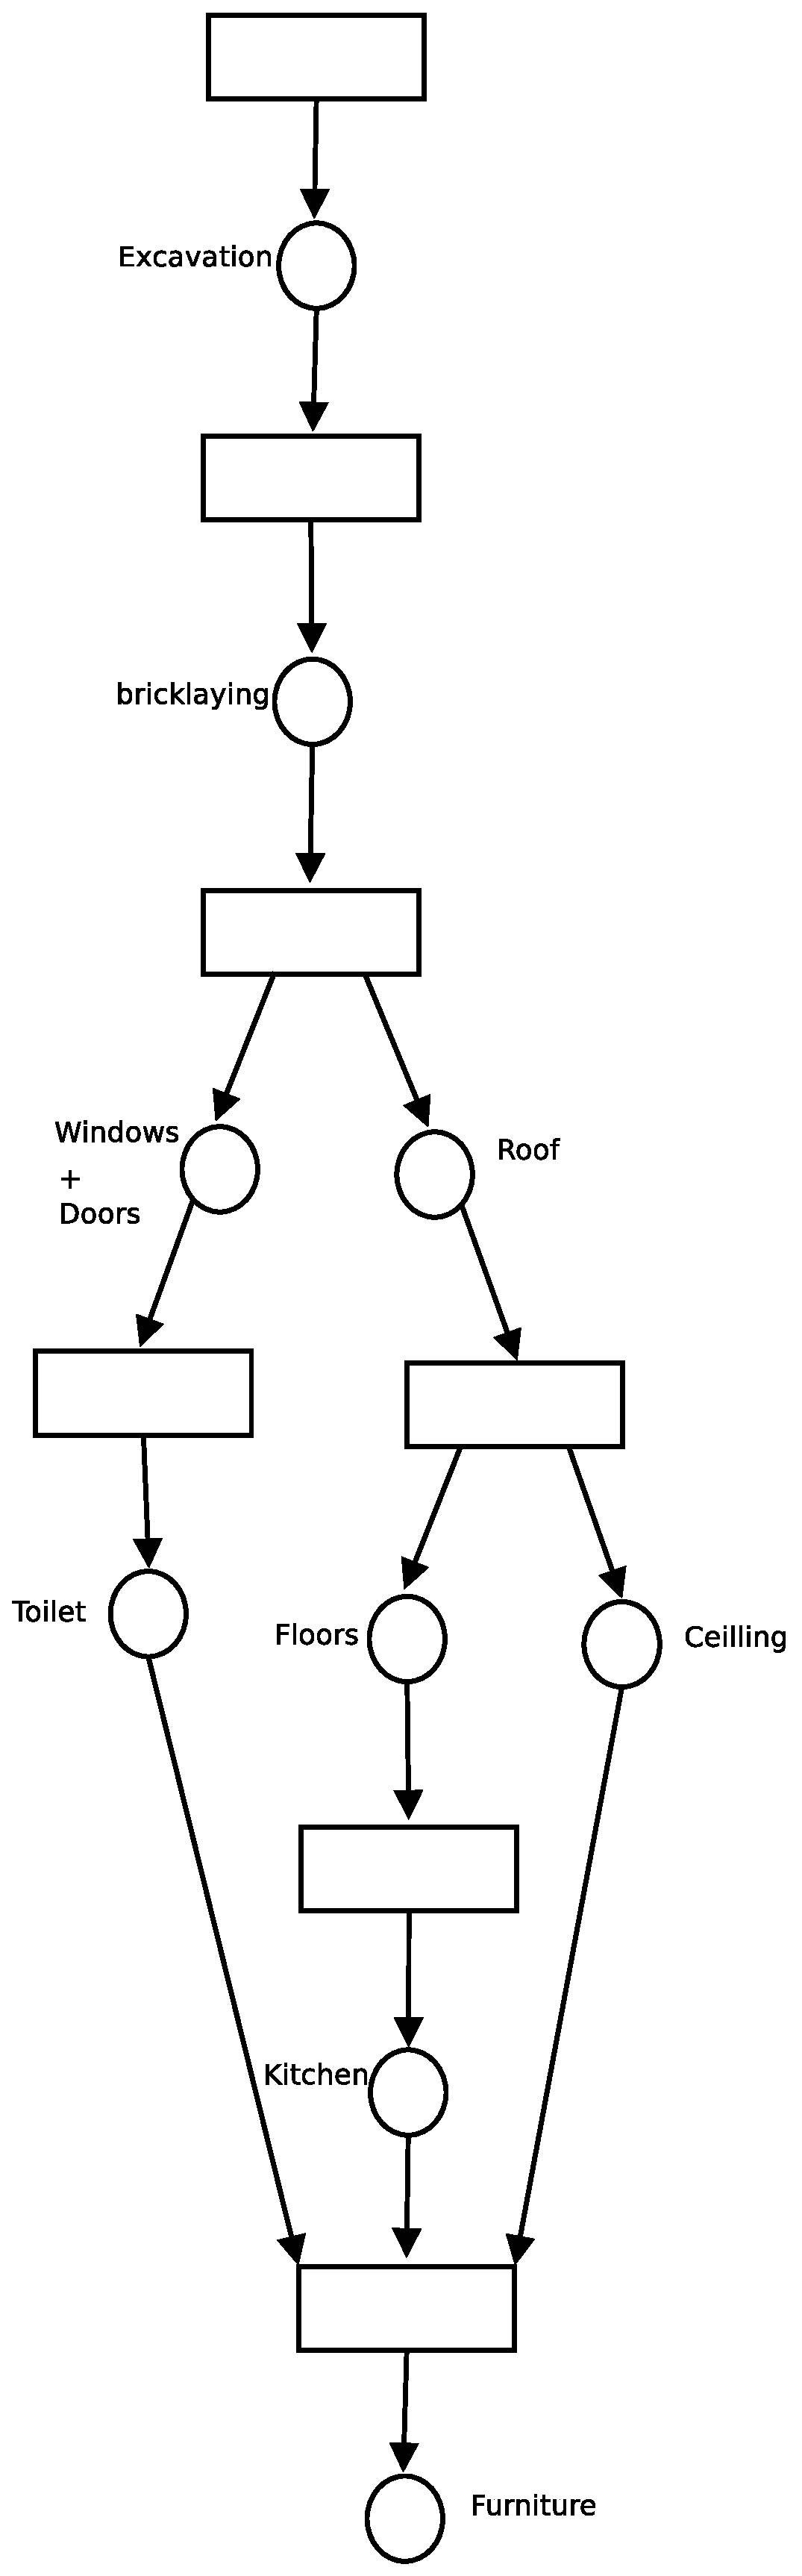
\includegraphics[height = 10cm]{exo42.eps} 
\caption{PT-net where each task is represented by a place}
\end{center} 
\end{figure}
\subsection*{Question 3}

Bien que les deux réseaux de pétri conservent la sémantique, le
deuxième semble plus naturel dans la mesure où l'on n'introduit pas
d'état artificiel d'entre-action. Modéliser les tâches par des places
convient donc mieux, les transitions servant à exprimer le passage
d'une tâche à l'autre, notamment la complétion d'une tâche.

\pagebreak
\section{Exercice 5}
\subsection{Question 1}
\subsection{Question 2}
\subsection{Question 3}

\pagebreak
\section{Exercice 6}
\subsection{Question 1}
\subsection{Question 2}

\pagebreak
\section{Exercice 7}
\subsection{Question 1}

TODO (below : just an example in tikz)

\begin{tikzpicture}[node distance=1.3cm,>=stealth',bend angle=45,auto]

  \tikzstyle{place}=[circle,thick,draw=blue!75,fill=blue!20,minimum size=6mm]
  \tikzstyle{red place}=[place,draw=red!75,fill=red!20]
  \tikzstyle{transition}=[rectangle,thick,draw=black!75,
  			  fill=black!20,minimum size=4mm]

  \tikzstyle{every label}=[red]

  \begin{scope}
    % First net
    \node [place,tokens=1] (w1)                                    {};
    \node [place] (c1) [below of=w1]                      {};
    \node [place] (s)  [below of=c1,label=above:$s\le 3$] {};
    \node [place] (c2) [below of=s]                       {};
    \node [place,tokens=1] (w2) [below of=c2]                      {};

    \node [transition] (e1) [left of=c1] {}
      edge [pre,bend left]                  (w1)
      edge [post,bend right]                (s)
      edge [post]                           (c1);

    \node [transition] (e2) [left of=c2] {}
      edge [pre,bend right]                 (w2)
      edge [post,bend left]                 (s)
      edge [post]                           (c2);

    \node [transition] (l1) [right of=c1] {}
      edge [pre]                            (c1)
      edge [pre,bend left]                  (s)
      edge [post,bend right] node[swap] {2} (w1);

    \node [transition] (l2) [right of=c2] {}
      edge [pre]                            (c2)
      edge [pre,bend right]                 (s)
      edge [post,bend left]  node {2}       (w2);
  \end{scope}

  \begin{pgfonlayer}{background}
    \filldraw [line width=4mm,join=round,black!10]
      (w1.north  -| l1.east)  rectangle (w2.south  -| e1.west);
  \end{pgfonlayer}
\end{tikzpicture}


\subsection{Question 2}

TODO (below : just an example in tikz)

\begin{tikzpicture}[node distance=1.3cm,>=stealth',bend angle=45,auto]

  \tikzstyle{place}=[circle,thick,draw=blue!75,fill=blue!20,minimum size=6mm]
  \tikzstyle{red place}=[place,draw=red!75,fill=red!20]
  \tikzstyle{transition}=[rectangle,thick,draw=black!75,
  			  fill=black!20,minimum size=4mm]

  \tikzstyle{every label}=[red]
 \begin{scope}[xshift=6cm]
    % Second net
    \node [place,tokens=1]
                      (w1')                                                {};
    \node [place]     (c1') [below of=w1']                                 {};
    \node [red place] (s1') [below of=c1',xshift=-5mm,label=left:$s$]      {};
    \node [red place,tokens=3]
                      (s2') [below of=c1',xshift=5mm,label=right:$\bar s$] {};
    \node [place]     (c2') [below of=s1',xshift=5mm]                      {};
    \node [place,tokens=1]
                      (w2') [below of=c2']                                 {};

    \node [transition] (e1') [left of=c1'] {}
      edge [pre,bend left]                  (w1')
      edge [post]                           (s1')
      edge [pre]                            (s2')
      edge [post]                           (c1');

    \node [transition] (e2') [left of=c2'] {}
      edge [pre,bend right]                 (w2')
      edge [post]                           (s1')
      edge [pre]                            (s2')
      edge [post]                           (c2');

    \node [transition] (l1') [right of=c1'] {}
      edge [pre]                            (c1')
      edge [pre]                            (s1')
      edge [post]                           (s2')
      edge [post,bend right] node[swap] {2} (w1');

    \node [transition] (l2') [right of=c2'] {}
      edge [pre]                            (c2')
      edge [pre]                            (s1')
      edge [post]                           (s2')
      edge [post,bend left]  node {2}       (w2');
  \end{scope}

  \begin{pgfonlayer}{background}
    \filldraw [line width=4mm,join=round,black!10]
      (w1'.north -| l1'.east) rectangle (w2'.south -| e1'.west);
  \end{pgfonlayer}
\end{tikzpicture}

\pagebreak
\section*{Exercice 8~: L'utilisation des réseaux de Pétri pour le
  contrôle des trains}
  
\emph{Nous suiverons ici le schema, qui représente 6 secteurs allant
  de 1 à 6, et non l'énoncé, qui évoque 7 secteurs de 1 à 7. Pour la
  question 3 les secteurs seront, par simplicité de notation, supposés
  numérotés de 0 à n et non de 1 à n+1.}

\subsection*{Question 1}

Chaque place pourra correspondre à un secteur, chaque jeton à un train
et chaque transition est un mouvement de train d'un secteur au
prochain secteur~:

\begin{center}
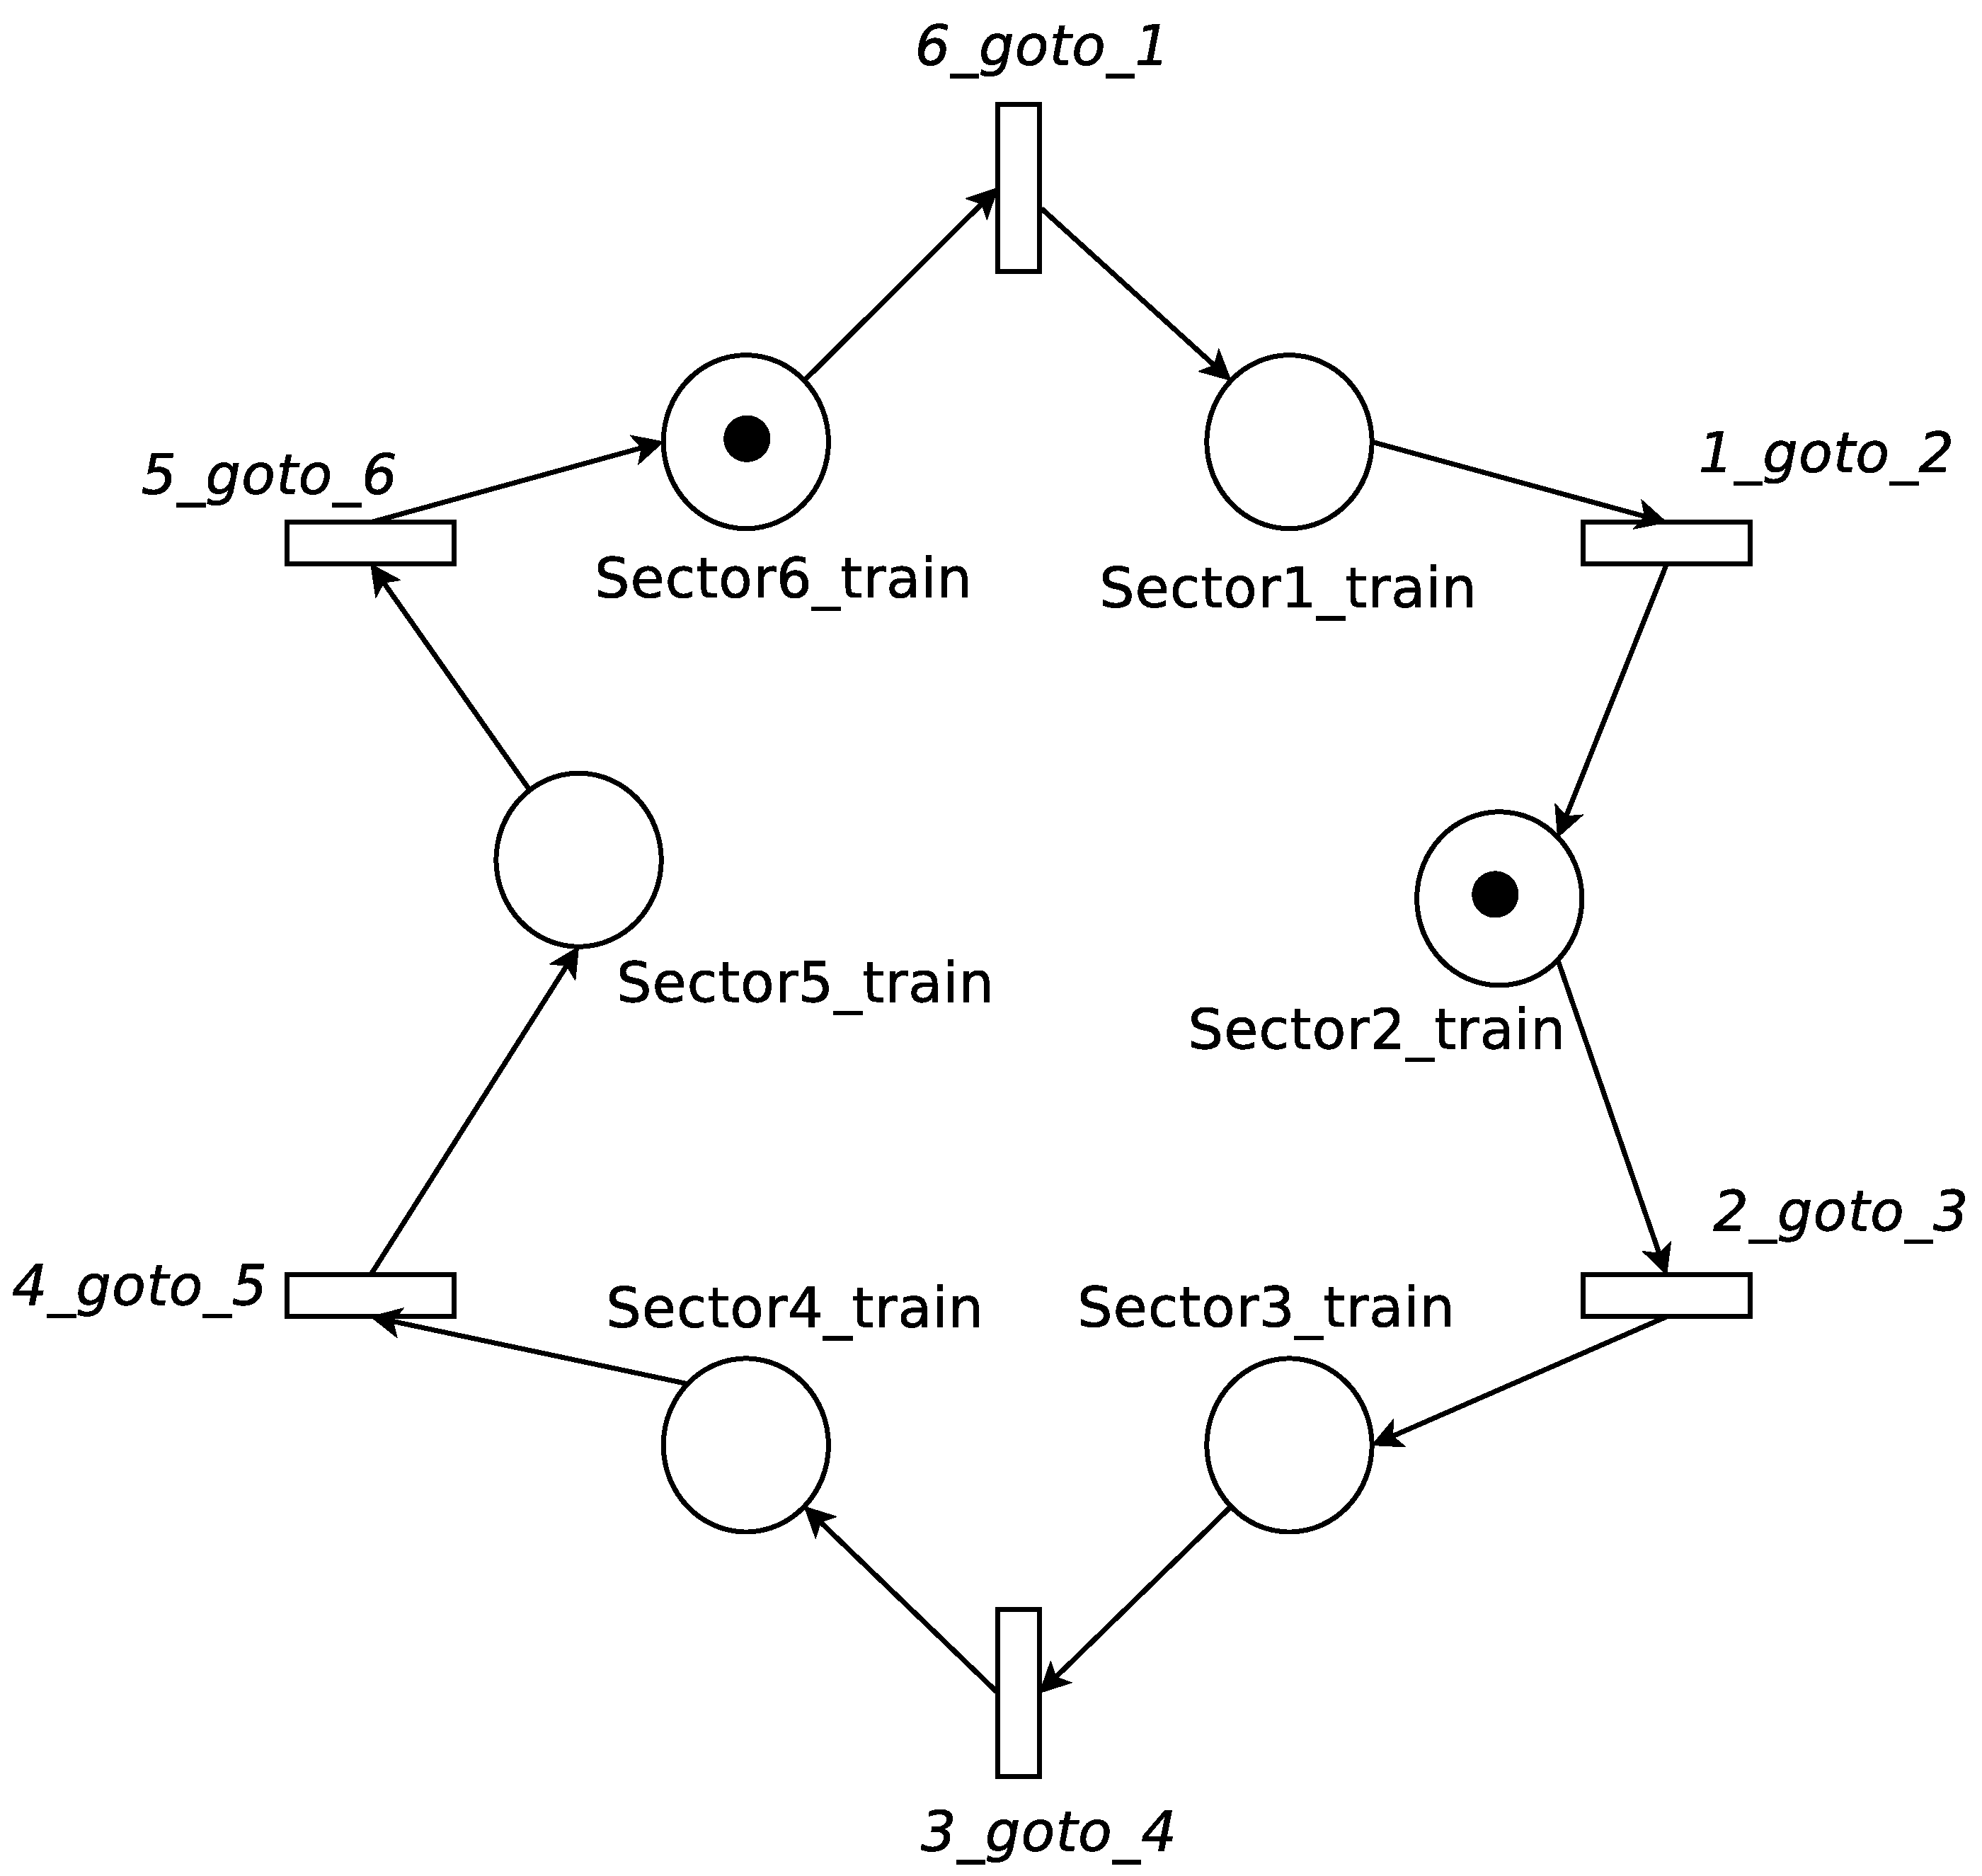
\includegraphics[height = 0.3\paperwidth]{exo8_1.eps}
\end{center}

Le réseau ci-dessus n'empêche cependant pas la collision de trains,
chose qu'il serait préférable d'éviter. Démunis d'arcs inhibiteurs,
nous nous devions de créer pour chaque secteur une place binaire dont
la présence d'un jeton correspond à la non présence de train dans ce
secteur.

\emph{Les parties ajoutées sont en vert~:}

\begin{center}
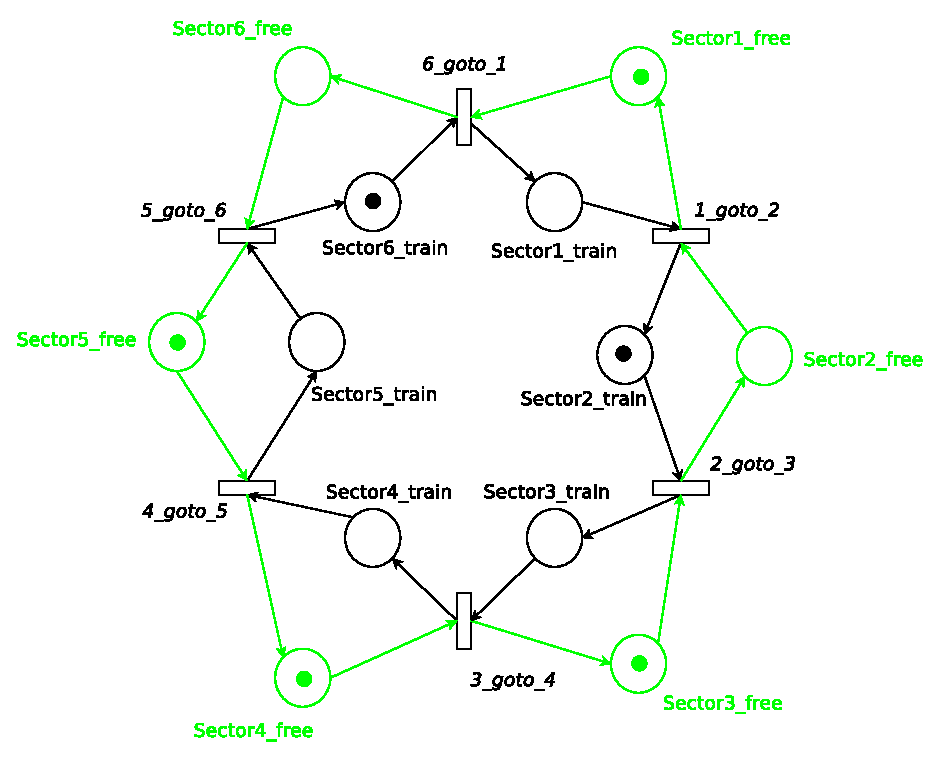
\includegraphics[height = 0.4\paperwidth]{exo8_2.eps}
\end{center}

Nous avons ainsi comme invariant qu'un secteur est toujours soit
libre, soit occupé par un seul et unique train. Il nous reste comme
condition à remplir que les secteurs adjacents à un secteur occupé
soient libres~:

\begin{center}
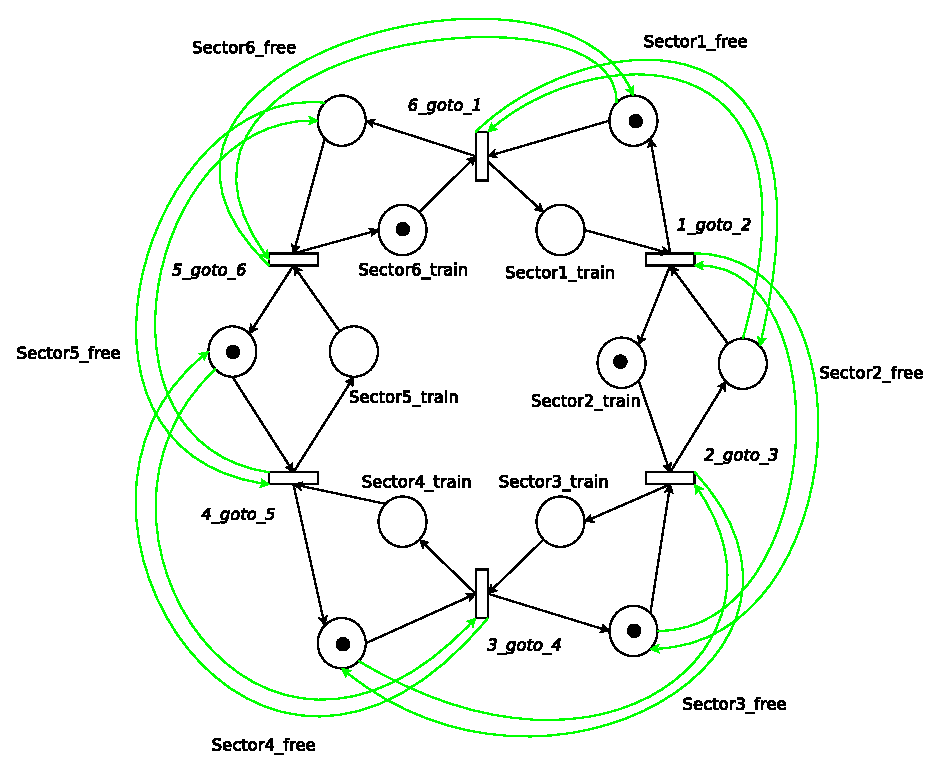
\includegraphics[height = 0.5\paperwidth]{exo8_3.eps}
\end{center}

Maintenant il faut différencier les deux trains, chose que nous
pouvons faire en recopiant le cycle interne de places.

\emph{Pour faciliter la lecture, les deux circuits analogiques pour
  les deux trains ont étés coloriés en rouge et en bleu
  respectivement~:}

\begin{center}
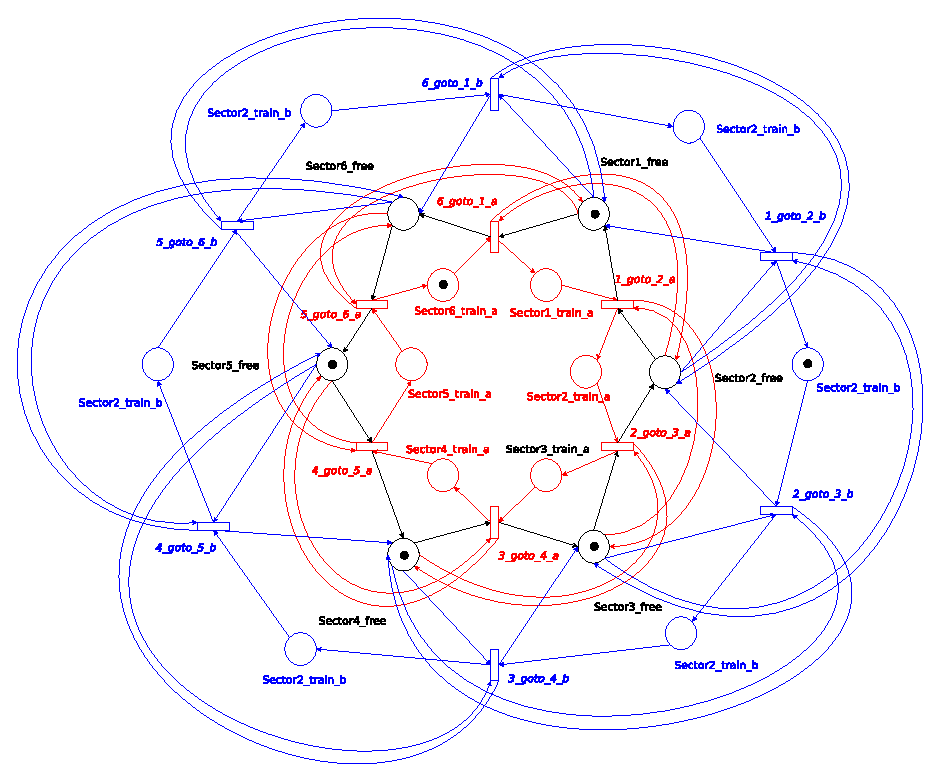
\includegraphics[height = 0.6\paperwidth]{exo8_uncoloured.eps}
\end{center}


\subsection*{Question 2}

En partant du réseau précédent et en écrasant les deux circuits
\og{}train\fg{} en un seul, nous nous retrouvons avec le réseau
colorié suivant.

\emph{Le jeton rouge représente le premier train, le bleu la deuxième, et ceux
noirs l'absence de train pour un secteur donné~:}

\begin{center}
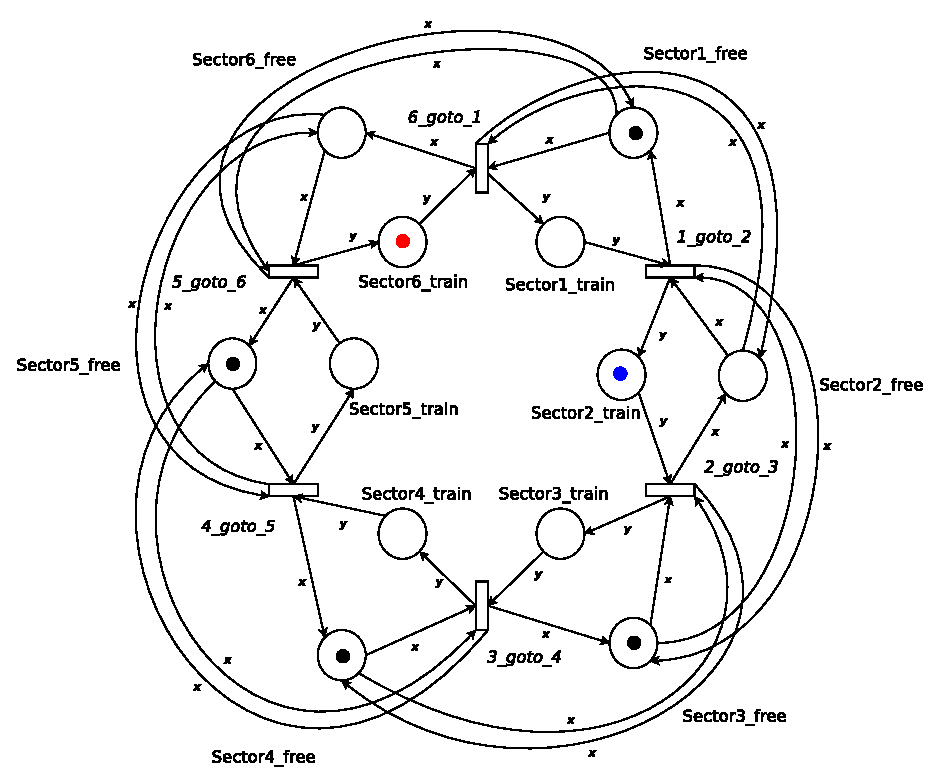
\includegraphics[height = 0.5\paperwidth]{exo8_coloured.eps}
\end{center}

Il est possible de simplifier ce réseau en écrasant les deux cycles ensemble. 
Ci-dessous un jeton noir correspond à la non-présence d'un train dans le secteur 
correspondant, un jeton d'une autre couleur à un train présent~:

\begin{center}
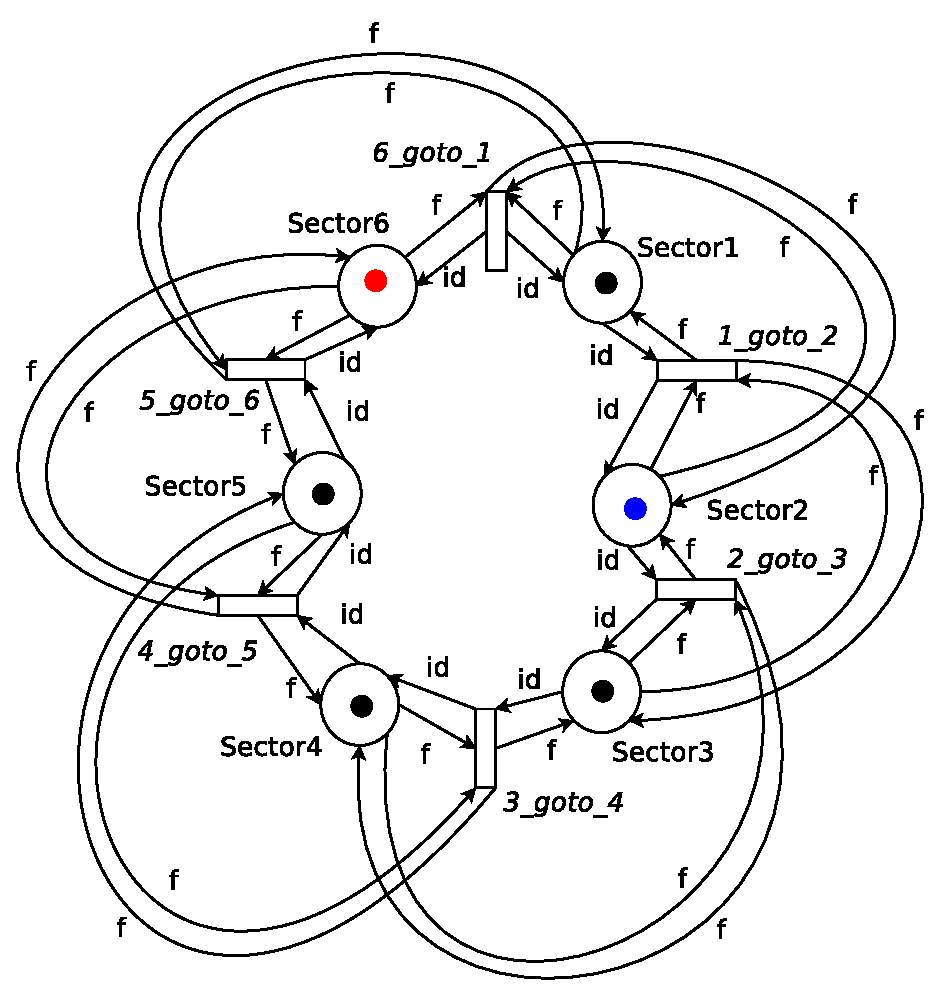
\includegraphics[height = 0.5\paperwidth]{exo8_coloured_2_v2.eps}
\end{center}

Où~:

$\forall c \in \{RED, BLUE\}$ $id(c) = c$

$\forall c \in \{RED, BLUE\}$ $f(c) = BLACK$

Ce réseau est beaucoup plus simple à aborder que la version
non-colorée, qui pour $n$ trains aura $n+1$ fois plus de places. Cela
étant sans la définition de la fonction $f$ (projection sur la couleur
noir) il n'est pas possible de comprendre le fonctionnement du
réseau~: le prix de la simplification du graphe est une augmentation
de la complexité des fonctions de transition.

Le premier réseau coloré semble un bon compromis entre les deux~: le
graphe a du sens sans information supplémentaire, mais reste un
facteur linéaire (en le nombre de trains) plus \og{}compact\fg{} que le réseau
non-coloré.


\subsection*{Question 3}

Soit le réseau suivant~:

\begin{center}
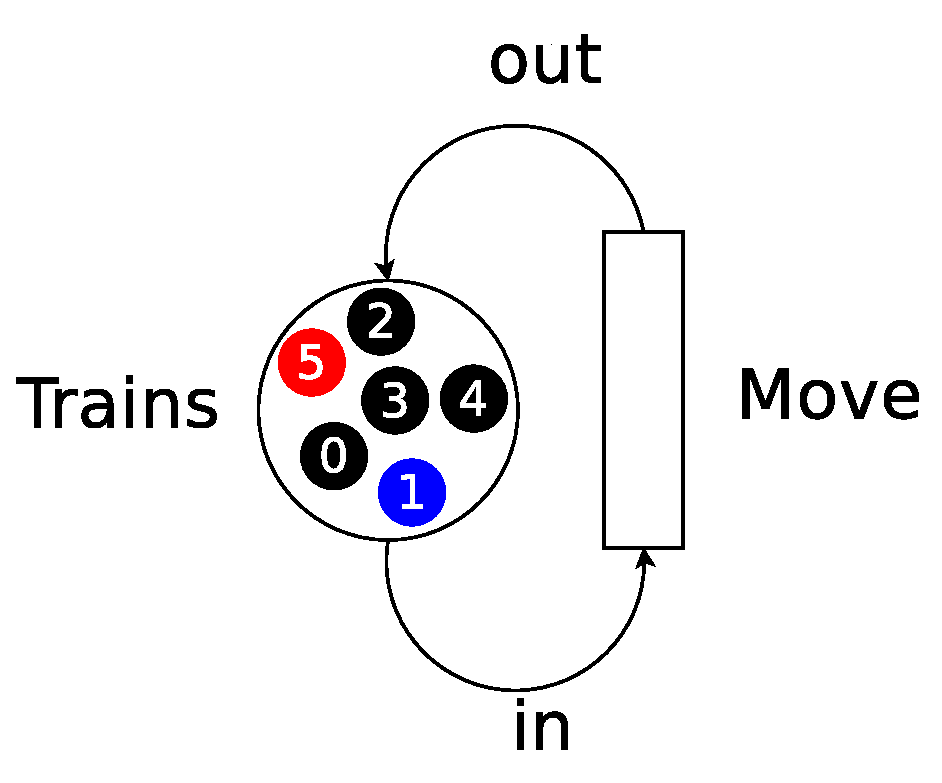
\includegraphics[height = 0.4\paperwidth]{exo8_coloured_3.eps}
\end{center}

Ici chaque couleur est une paire $c \in Trains \cup NULL \times Sectors$. 
Pour l'exemple~:

$Trains = \{ A, B\}$

$Sectors = \{0, \ldots{}, 5\}$

Les secteurs sont notés à partir de 0 et non 1 pour permettre la plus simple 
utilisation des modulo. 
Posons d'ailleurs $n\oplus{m} = (n+m)\mod{\left|Sectors\right|}$. 
Nous avons $5\oplus{1} = 0$ pour l'exemple.

$c = (T, i)$ sera noté $T_i$ par la suite. Il nous suffit de définir maintenant 
$in$ et $out$ de manière à ce que le réseau ait tous les propriétés souhaités.

Soit~:

$in(T_i) = T_{i} + NULL_{i\oplus{1}} + NULL_{i\oplus{2}}$

Et~:

$out(T_i) = NULL_{i} + T_{i\oplus{1}} + NULL_{i\oplus{2}}$

Avec bien sur $dom(in) = dom(out) = Trains \times Sectors$. Autrement dit 
$\forall i$, $in(NULL_i)$ et $out(NULL_i)$ non-définis.

\pagebreak
\section{Exercice 9}
\subsection{Question 1}

\begin{center}
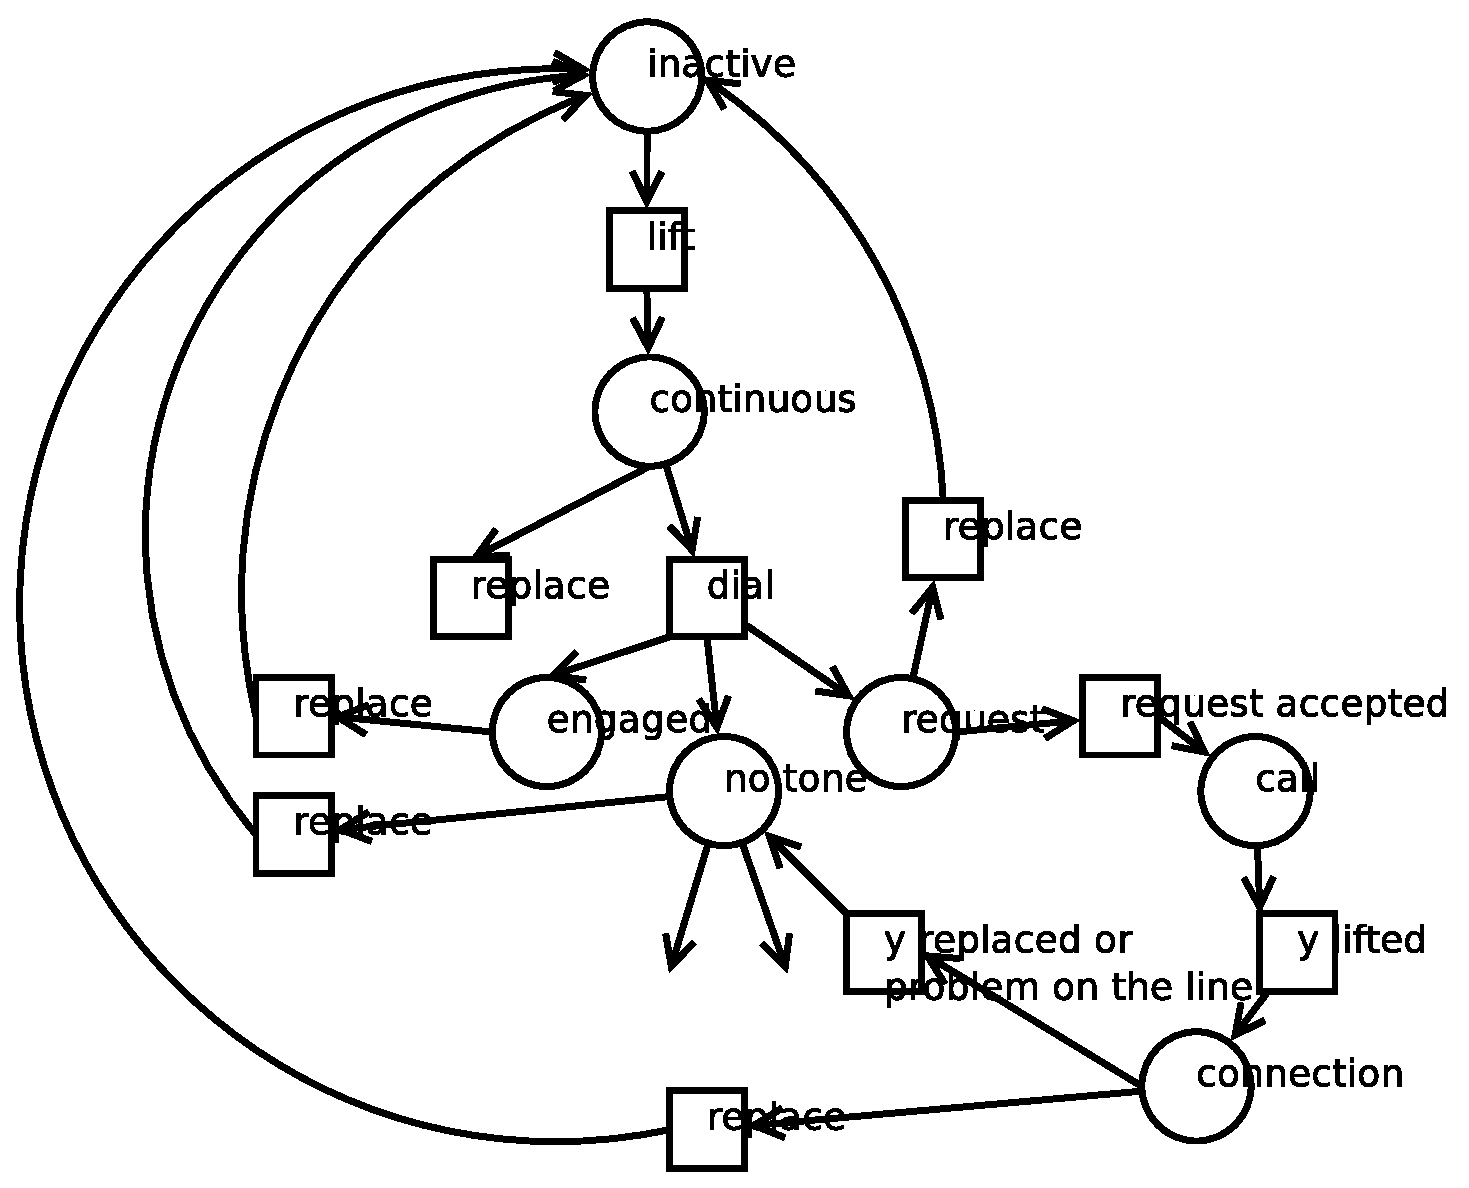
\includegraphics[height = 8cm]{exo9_1.eps}
\end{center}

\subsection{Question 2}

Quand un téléphone appelle son propre numéro, il tombe directement dans l'état \textbf{engaged}.

Le téléphone appelé peut mettre fin à la conversation, le téléphone
appelant tombe alors dans l'état \textbf{no tone}.

Ce modèle est effectif en France, mais il demeure basique : un certain
nombre de fonctionnalités <<~modernes~>> manquent à l'appel. Ainsi,
c'est le cas du rappel automatique en cas de correspondant occupé, ou
de la mise en attente.

\subsection{Question 3}

Pour représenter le caractère activé ou désactivé d'un numéro de
téléphone, nous proposons de rajouter deux couleurs \textit{activé}
$a$ et \textit{désactivé} $d$.

Le modèle correspondant est le suivant~:

\begin{center}
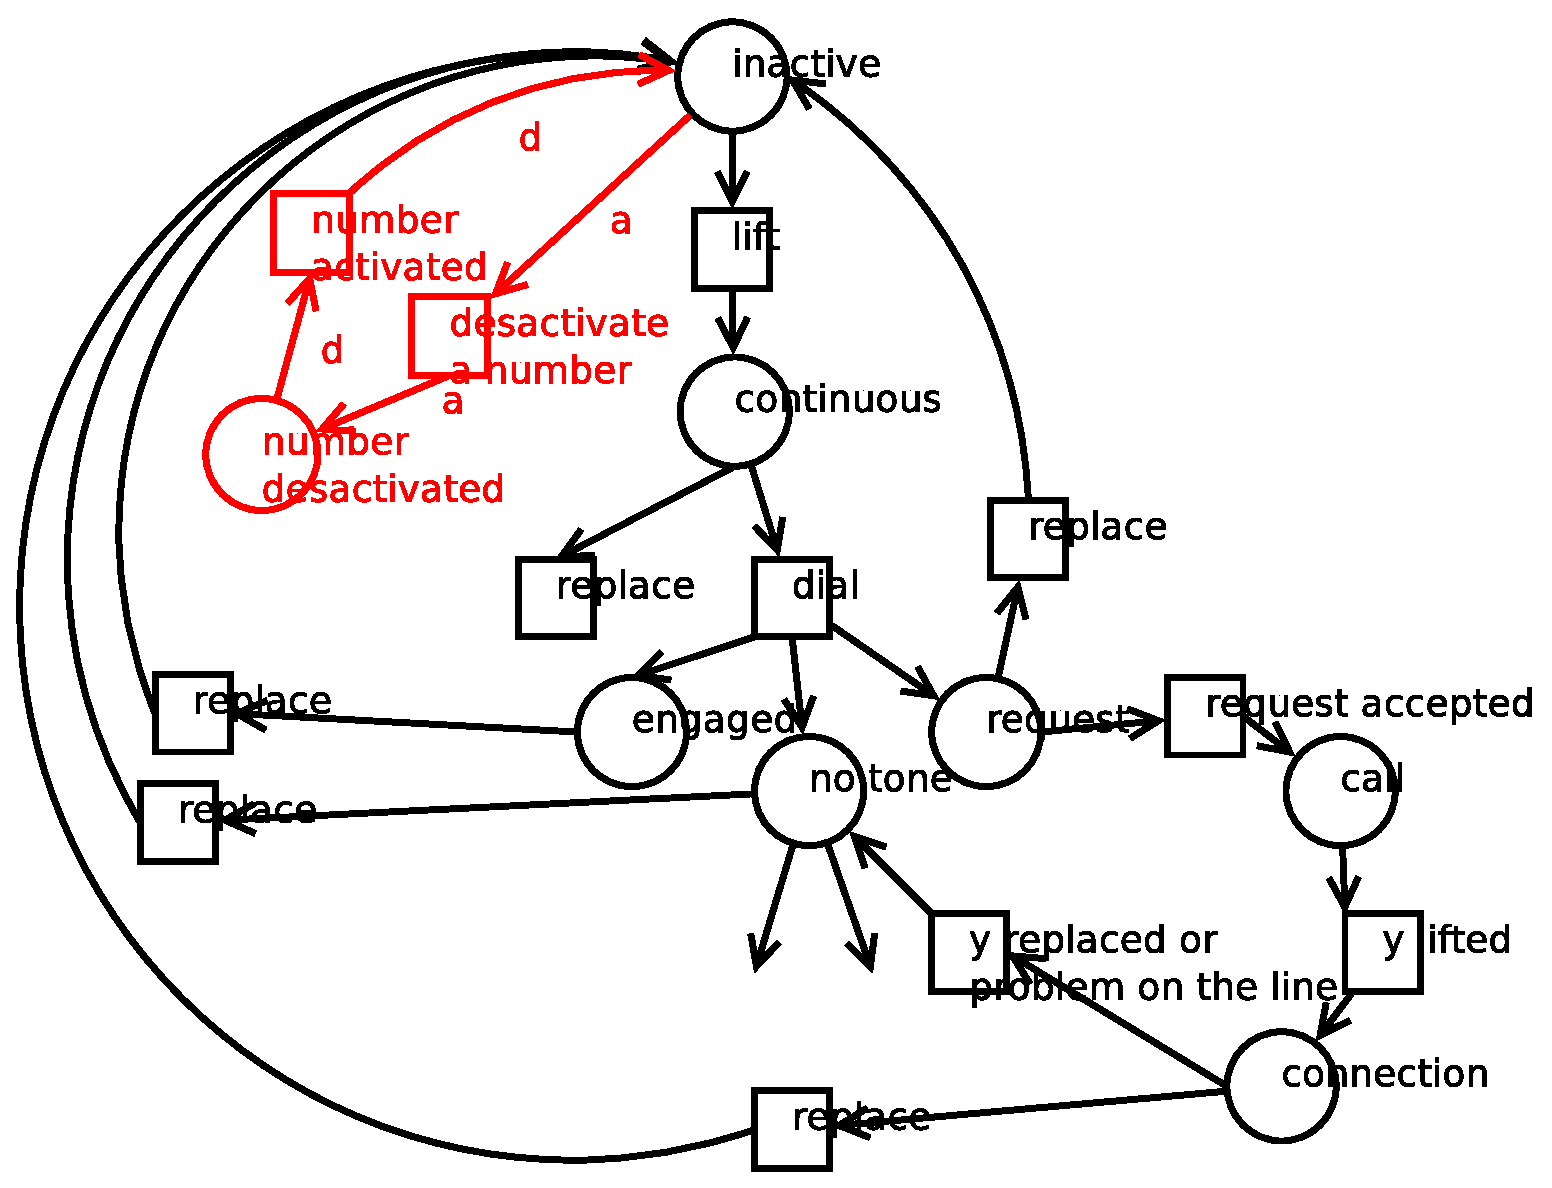
\includegraphics[height = 8cm]{exo9_2.eps}
\end{center}
\subsection{Question 4}

Afin de tenir compte des dépassements de délai, on transforme le
réseau de pétri en réseau de pétri temporisé de la manière suivante~:

Le temps est exprimé en secondes.

\begin{center}
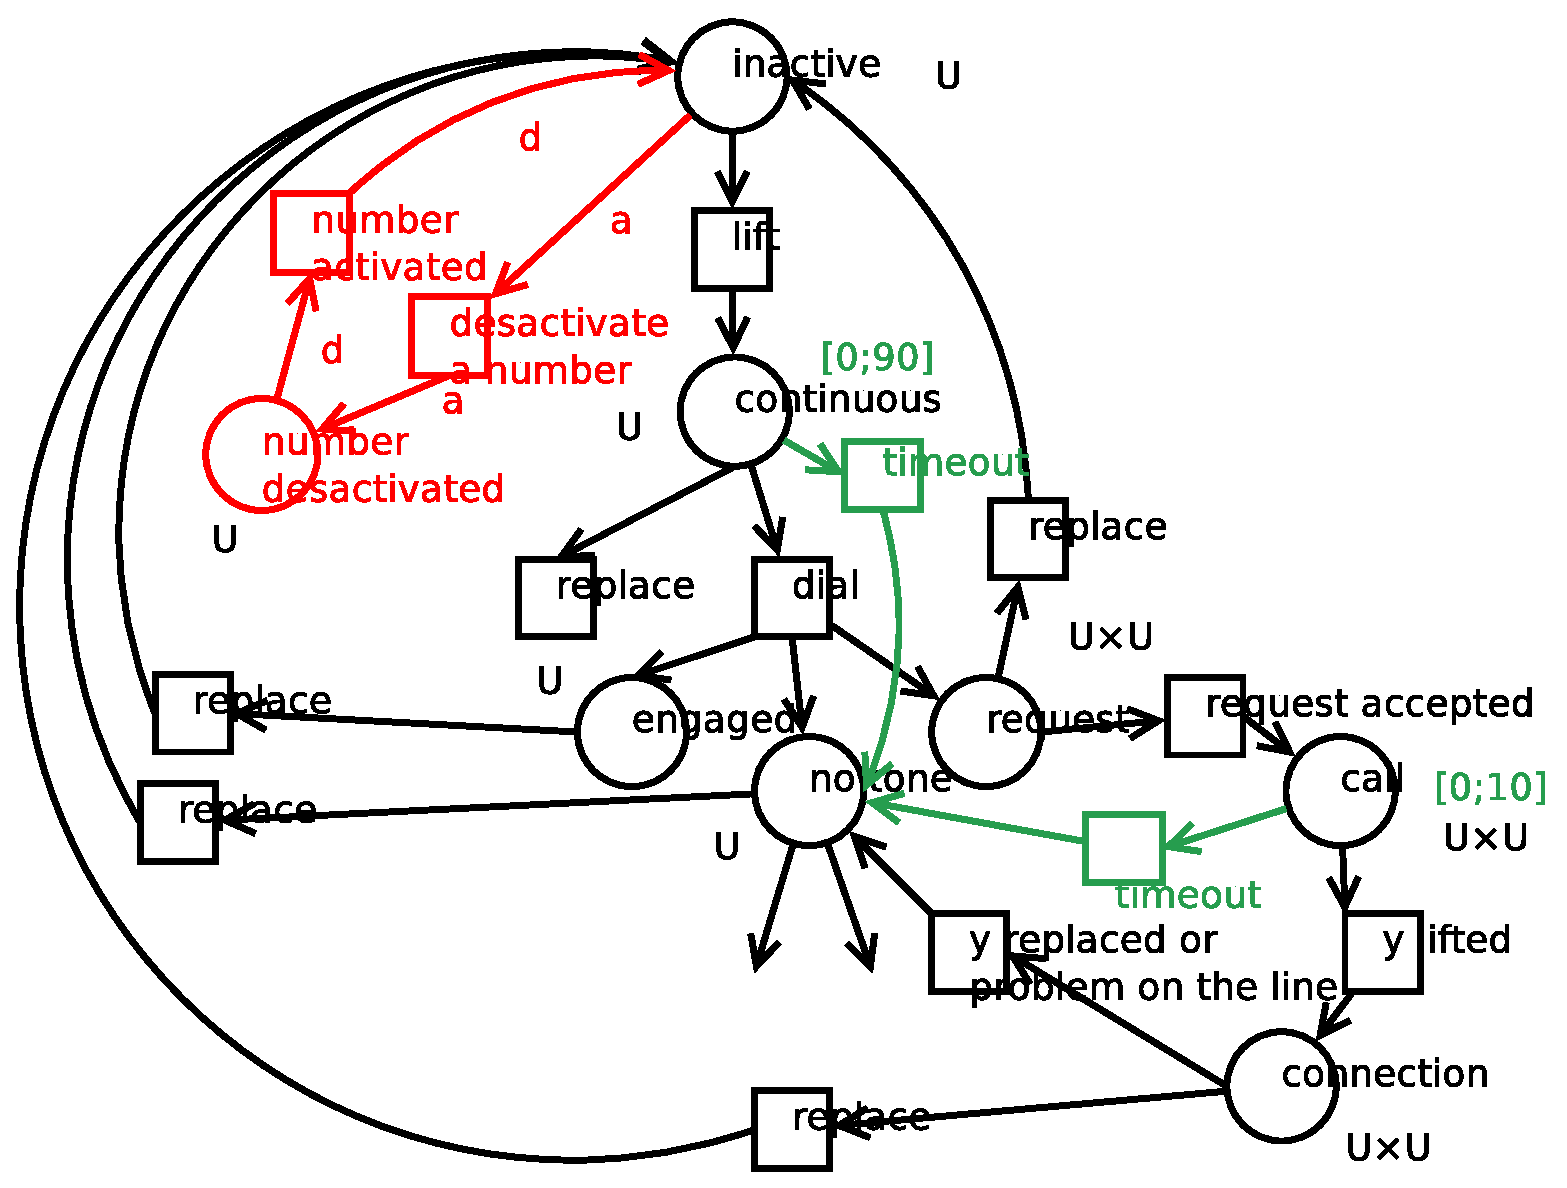
\includegraphics[height = 8cm]{exo9_3.eps}
\end{center}


\end{document}
